%Technische Mitarbeiter und Sekretariat
%Technical staff and office
\newpage

\section*{Technische Mitarbeiter und Sekretariat}

\begin{figure}[htbp]
	% minipage mit (Blind-)Text
	\begin{minipage}[t]{0.18\textwidth} 
	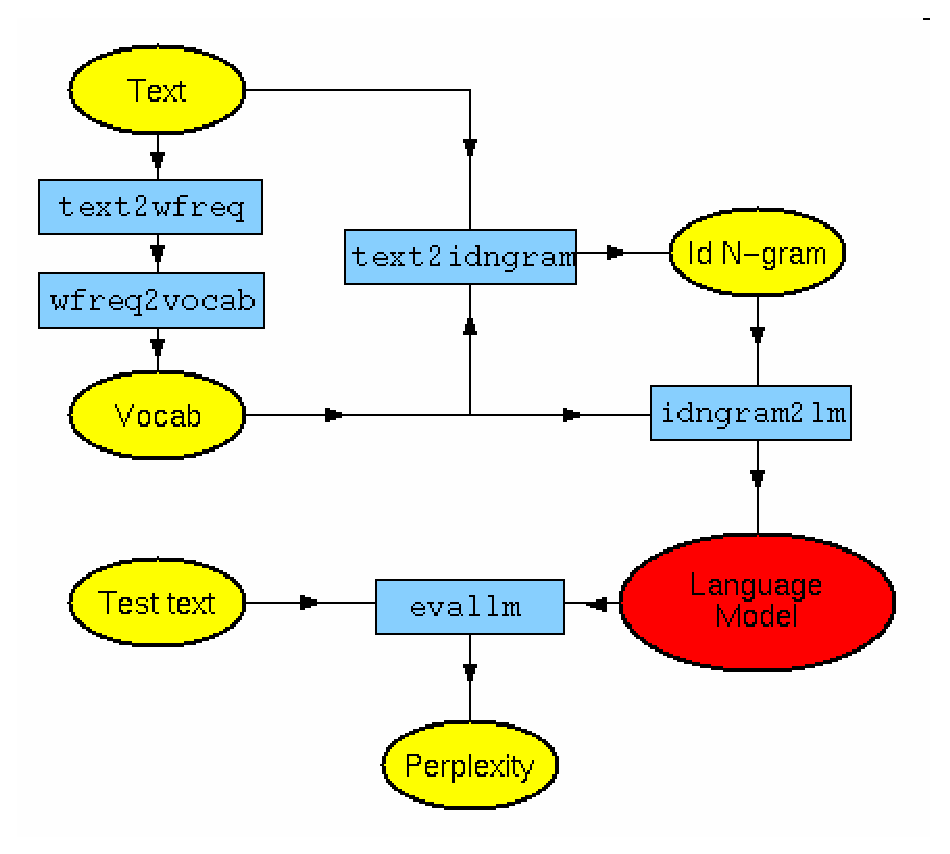
\includegraphics[width=\textwidth]{Bilder/toolkit.eps}
	%\caption{Eine Grafik}
	%\label{Bild}
	\end{minipage}
	% Auff�llen des Zwischenraums
	\hfill
	% minipage mit Grafik
	\begin{minipage}[b]{0.3\textwidth}
	% \textwidth bezieht sich nun auf die Minipage
 	\makebox[0.3\textwidth][l]{	\scriptsize{Dipl.-Ing Helmut Foth}	}\\
 	\makebox[0.3\textwidth][l]{	\scriptsize{Laboringenieur}	}\\
 	\makebox[0.3\textwidth][l]{	\scriptsize{Electrical engineering master}}\\
 	\makebox[0.3\textwidth][l]{	\scriptsize{Mitarbeit seit:1995}}\\		
 

 	
	% \caption{Der Text}
	% \label{Text}
	\end{minipage}
	\hfill
	% minipage mit (Blind-)Text
	\begin{minipage}[b]{0.18\textwidth} 
	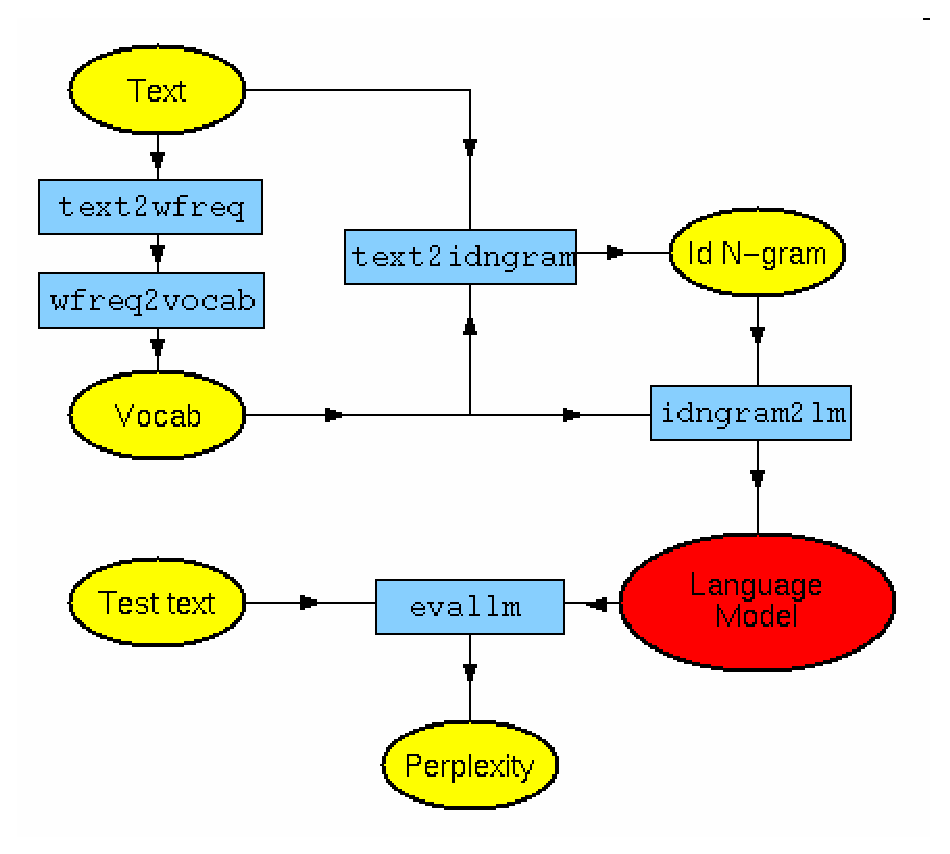
\includegraphics[width=\textwidth]{Bilder/toolkit.eps}
	%\caption{Eine Grafik}
	%\label{Bild}
	\end{minipage}
	% Auff�llen des Zwischenraums
	\hfill
	% minipage mit Grafik
	\begin{minipage}[b]{0.3\textwidth}
	% \textwidth bezieht sich nun auf die Minipage
 	\scriptsize{Title}\\
 	\parbox[b]{\textwidth}{
 	\scriptsize{Laboringenieur}	\\
 	\scriptsize{Electrical engineering technican}\\
 	\scriptsize{Mitarbeit seit:1995}\\	
 	}
	% \caption{Der Text}
	% \label{Text}
	\end{minipage}
% \caption{noch eine Caption}
\end{figure}


\begin{figure}[htbp]
	% minipage mit (Blind-)Text
	\begin{minipage}[b]{0.2\textwidth} 
	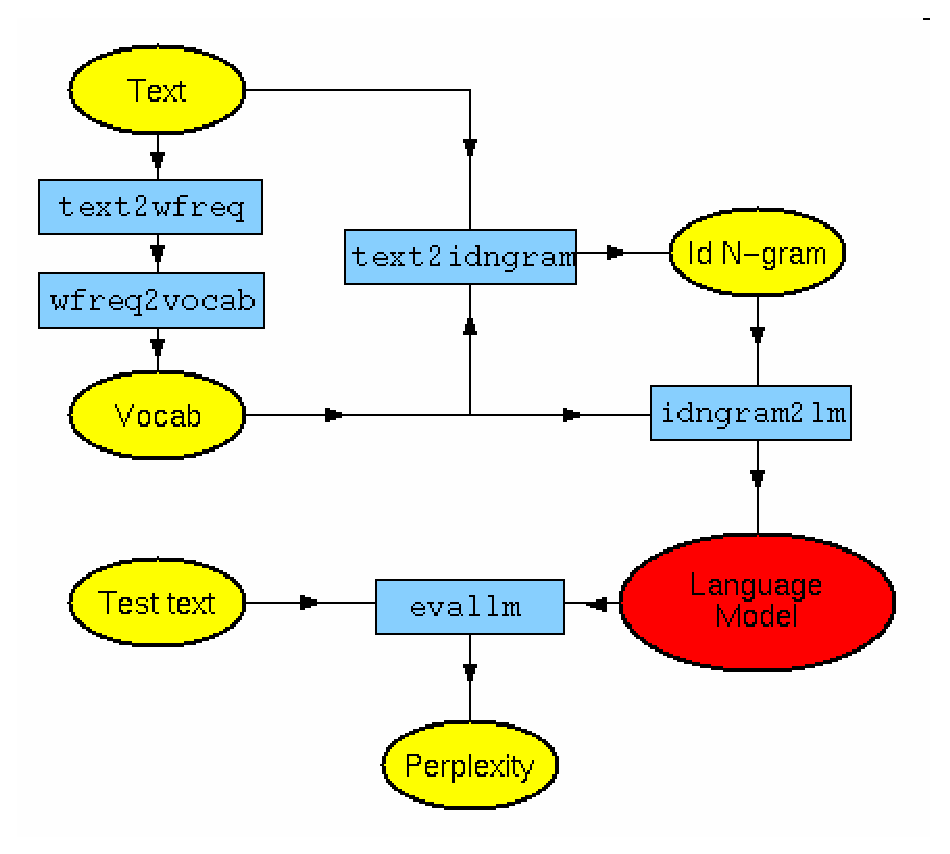
\includegraphics[width=\textwidth]{Bilder/toolkit.eps}
	%\caption{Eine Grafik}
	%\label{Bild}
	\end{minipage}
	% Auff�llen des Zwischenraums
	\hfill
	% minipage mit Grafik
	\begin{minipage}[b]{0.25\textwidth}
	% \textwidth bezieht sich nun auf die Minipage
 	Title\\
 	Job\\
 	Mitarbeit seit:1995\\	
	% \caption{Der Text}
	% \label{Text}
	\end{minipage}
	\hfill
	% minipage mit (Blind-)Text
	\begin{minipage}[b]{0.2\textwidth} 
	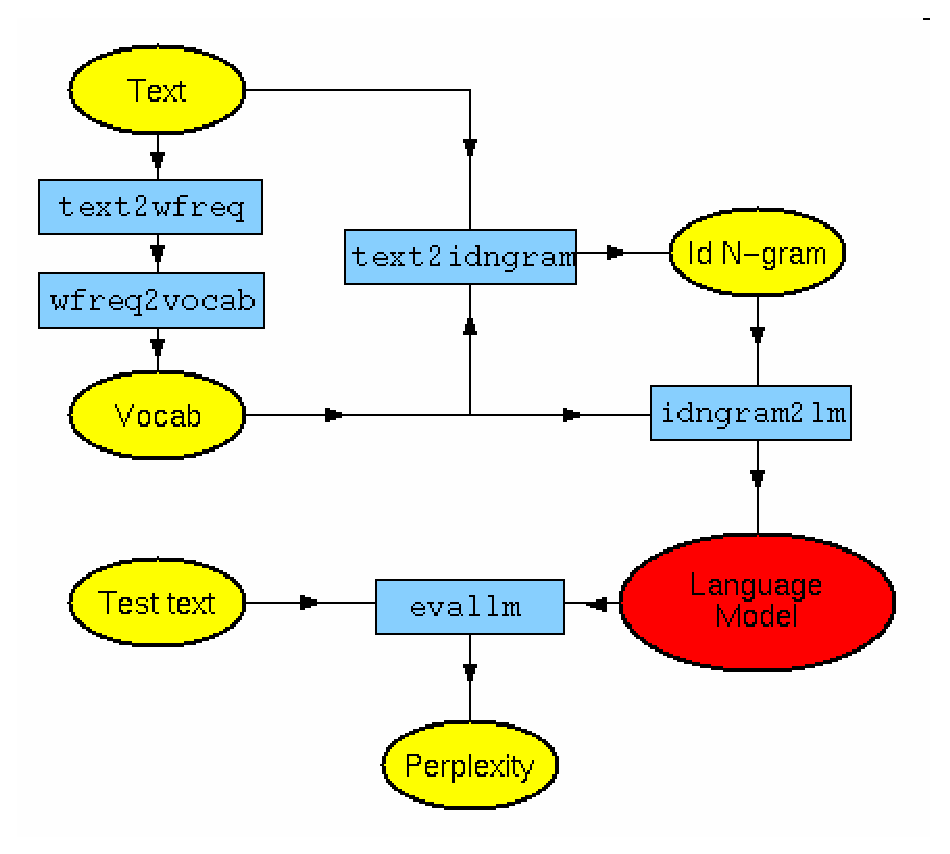
\includegraphics[width=\textwidth]{Bilder/toolkit.eps}
	%\caption{Eine Grafik}
	%\label{Bild}
	\end{minipage}
	% Auff�llen des Zwischenraums
	\hfill
	% minipage mit Grafik
	\begin{minipage}[b]{0.25\textwidth}
	% \textwidth bezieht sich nun auf die Minipage
 	Title\\
 	Job\\
 	Mitarbeit seit:1995\\	
	% \caption{Der Text}
	% \label{Text}
	\end{minipage}
% \caption{noch eine Caption}
\end{figure}
